\begin{frame}
  \PN Ya que la máquina $M_{i}$ puede tener uno o dos estados finales, la representaremos de la siguiente manera:
  \begin{figure}[h]
    \centering
    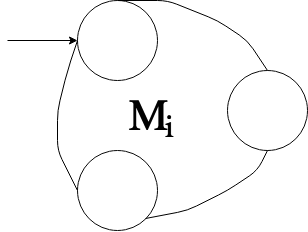
\includegraphics[scale=0.4]{graphics/figure_5.png}
  \end{figure}
  \begin{itemize}
    \item Si $M_{i}$ tiene \textbf{un solo estado final}, este está representado por el círculo de abajo a la izquierda
    \item Si $M_{i}$ tiene \textbf{dos estados finales}, el estado final de la derecha corresponde al estado $q_{si}$ y
      el de la izquierda abajo al estado $q_{no}$.
  \end{itemize}
\end{frame}
